%-------------------------------------------------------------------------------
% seq64_menu
%-------------------------------------------------------------------------------
%
% \file        seq64_menu.tex
% \library     Documents
% \author      Chris Ahlstrom
% \date        2015-08-31
% \update      2017-04-25
% \version     $Revision$
% \license     $XPC_GPL_LICENSE$
%
%     Provides the Menu section of seq24-user-manual.tex.
%
%-------------------------------------------------------------------------------

\section{Menu}
\label{sec:seq64_menu}

   The \textsl{Sequencer64} menu, as seen at the top of
   \figureref{fig:seq64_main_screen}, is fairly simple, but it is important to
   understand the structure of the menu entries.

\subsection{Menu / File}
\label{subsec:seq64_menu_file}

   The \textbf{File} menu is used to save and load standard MIDI files.
   \textsl{Sequencer64} will handle any Format 0 or
   Format 1 standard files that other sequencers export.
   The \textsl{Sequencer64} menu entry contains the sub-items shown in
   \figureref{fig:seq64_menu_file_items}.  The next few sub-sections discuss
   the sub-items in the \textsl{File} sub-menu.

\begin{figure}[H]
   \centering 
   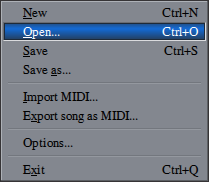
\includegraphics[scale=1.00]{menu/menu_file.png}
   \caption{Sequencer64 File Menu Items}
   \label{fig:seq64_menu_file_items}
\end{figure}

   \begin{enumber}
      \item \textbf{New}
      \item \textbf{Open...}
      \item \textbf{Save}
      \item \textbf{Save As...}
      \item \textbf{Import MIDI...}
      \item \textbf{Export song as MIDI...}
      \item \textbf{Options...}
      \item \textbf{Exit}
   \end{enumber}

\subsection{Menu / File / New}
\label{subsec:menu_file_new}

   The \textbf{New} menu entry clears out any current song and patterns,
   allowing one to create new ones from scratch.
   If unsaved changes are pending, the user will be prompted to save the
   changes.  Prompting for changes is more comprehensive than \textsl{Seq24}.

\subsubsection{Menu / File / Open}
\label{subsubsec:seq64_menu_file_open}

   The \textbf{Open} menu entry opens a song (MIDI file)
   that had been saved previously.  It opens up a standard GTK+2 file dialog:

\begin{figure}[H]
   \centering 
   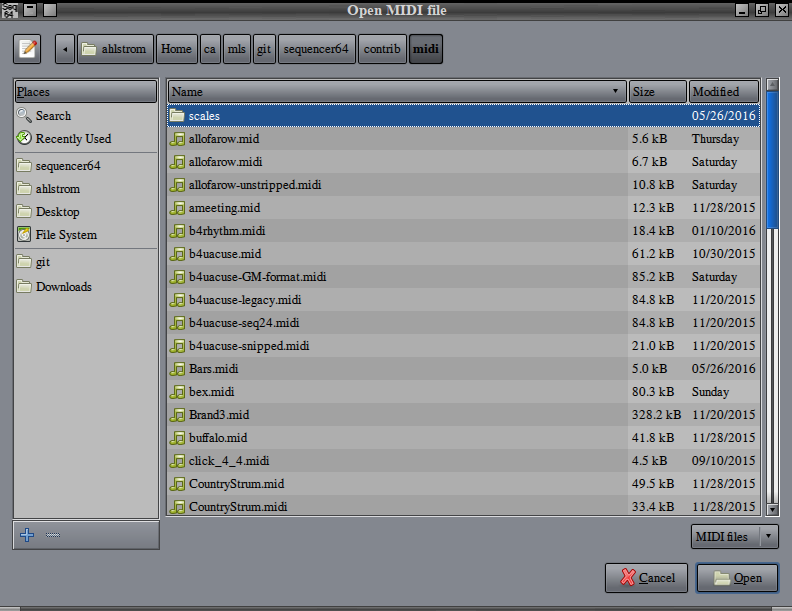
\includegraphics[scale=0.65]{menu/menu_file_open.png}
   \caption{File / Open}
   \label{fig:seq64_menu_file_open}
\end{figure}

   This dialog lets one type a file-name, highlighting the first file (if any)
   that matches the characters typed so far.

   If unsaved changes are pending, the user will (usually)
   be prompted to save the changes.
   When in doubt, save!  If still in doubt, keep backups of your tunes!

\subsubsection{Menu / File / Save and Save As}
\label{subsubsec:menu_file_open_save_as}

   The \textbf{Save} menu entry saves the song under its current file-name.
   If there is no current file-name, then it opens up a standard file
   dialog to name and save the file.

   The \textbf{Save As} menu entry saves a song under a different name.
   It opens up the following standard file dialog, very similar to the 
   \textbf{File Open} dialog, with an additional \textbf{Name} text-edit field.

\begin{figure}[H]
   \centering 
   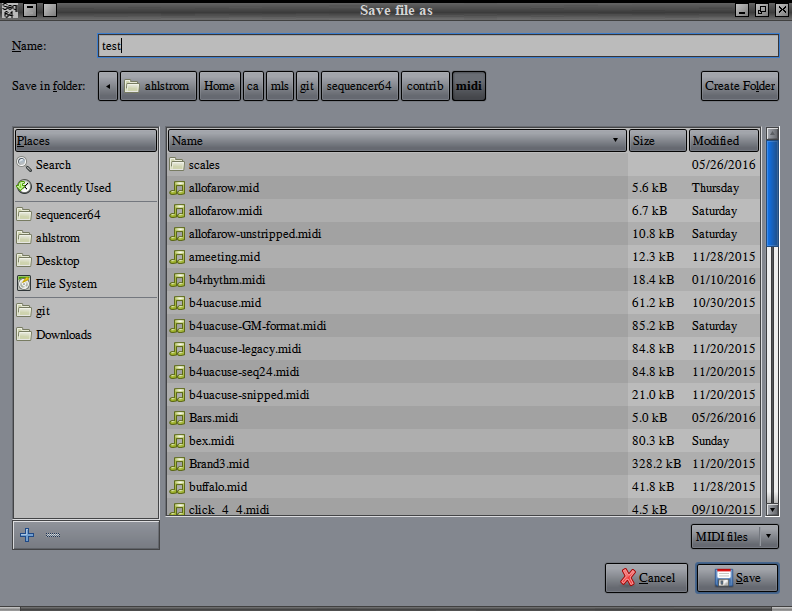
\includegraphics[scale=0.65]{menu/menu_file_save_as.png}
   \caption{File / Save As}
   \label{fig:seq64_menu_file_save_as}
\end{figure}

   To save a new file, or to save the current existing file to a new name,
   enter the name in the name field, without an extension.
   \textsl{Sequencer64} will append a \texttt{.midi} extension to the filename.
   The file will be saved in a format that the Linux \textsl{file} command
   will tag as something like:

   \begin{verbatim}
      myfile.midi: Standard MIDI data (format 1) using 16 tracks at 1/192
   \end{verbatim}

   It looks like a simple MIDI file, and yet, if one re-opens it in
   \textsl{Sequencer64}, one sees that all of the labelling, pattern information,
   and song layout has been preserved in this file.
   Even the pattern layout (arrangement), as discussed in
   \sectionref{subsubsec:seq64_song_editor_arrangement_panel_roll},
   have been saved.
   (But the L and R marker positions are not saved.)

   Compare the sizes of the original project MIDI file
   and the output MIDI file after \textsl{Sequencer64} saves them
   are different.
   The reason is that, after the last track in the file, a number of
   sequencer-specific (SeqSpec) items are saved, to preserve this extra
   information.  In legacy mode, \textsl{Sequencer64} saves this information
   in the same format as \textsl{Seq24}. Otherwise, it saves it
   in an even more MIDI-compatible format.  There is also an option to strip
   this extra information if it is empty.

   \textbf{New:}
   \index{new!seqspec format}
   In its normal mode, \textsl{Sequencer64} saves this
   information by marking each SeqSpec section
   as vendor-specific information, and marking this section as a regular
   MIDI track.
   The legacy and new formats of the final "track" are explained in
   \sectionref{subsec:legacy_midi_format}.

\subsubsection{Menu / File / Import MIDI}
\label{subsubsec:seq64_menu_file_import}

   The \textbf{Import} menu entry allows one to import an SMF 0
   or SMF 1 MIDI file into one or more patterns, one pattern per track in
   the MIDI file.  Even long tracks, that aren't short loops, are read in
   properly.

\begin{figure}[H]
   \centering 
   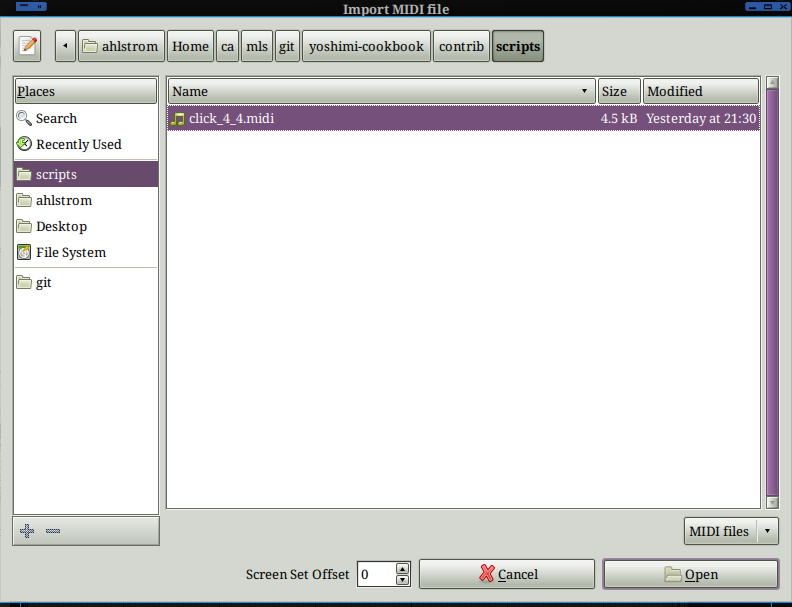
\includegraphics[scale=0.65]{menu/menu_file_import.png}
   \caption{File / Import MIDI}
   \label{fig:seq64_menu_file_import}
\end{figure}

   When imported, each track, whether a music track or an information track,
   is entered into its own loop/pattern box.  The import operation can
   handle reasonably complex files,
%  as shown in the following diagram, which shows an import of
   such as the \texttt{contrib/b4uacuse.mid} file, which contains
   a transcription of an Eric Clapton / Robert Cray tune made over 20 years ago.
%  and had uploaded to the \textsl{GEnie} network service.

   Note the additional file-dialog field,
   \textbf{Select Screen Offset}.
   \index{import!select screen offset}
   \index{select screen offset}
   This setting lets one place the imported data into a screen-set other than
   the first screen-set (screen-set 0).
   This field is not editable.  It requires using the scroll button to move the
   screen set offset up or down in value.  The legal values range from 0
   to 31.

   When the file is imported, the sequence number for each track read in is
   adjusted to put the track in the desired screen-set.
   The import can placed the imported data into any of the 32 available
   screen-sets.  Quite large songs can be built up by importing patterns from
   other MIDI files.

   The import operation also handles SMF 0 MIDI files.  It parcels out the SMF
   0 into sequences/patterns for each of the 16 MIDI channels.  It also puts
   all of the MIDI data into the 17th pattern (pattern 16), in case it is
   needed.  Note that this slot is used no matter which screen-set one imports
   the file into.  Bug, or feature?

\subsubsection{Menu / File / Export song as MIDI}
\label{subsubsec:seq64_menu_file_export}

   Thanks to the \textsl{Seq32} project, the ability to export songs to MIDI
   format has been added.
   "But wait,", you say, "Sequencer64 already saves to a MIDI-compatible
   format.  Why the need for an Export function?"
   Well, the \textbf{Export song as MIDI} function modifies the song in the
   following ways:

   \begin{itemize}
      \item Only tracks (sequences, loops, or patterns)
         \index{exportable}
         that are "exportable" are written.  To be exportable, a
         track must be unmuted, and it must have triggers (see
         \sectionref{subsubsec:concepts_terms_trigger}).  That is,
         the track must have a layout entry in the \textbf{Song Editor}.
         A track need not have any playable data to be exported.
      \item All of the triggers for a given track are consolidated.  Each
         trigger is used to generate the events, including repeats and offsets
         play of the track information.  If there is a gap in the layout (e.g.
         due to the \textbf{Expand} operation in the Song Editor), then there
         is a corresponding gap in the events that are played. The result is
         one consolidated trigger that reconstructs the original playback
         layout.  This trigger is not needed (or even usable) in any
         non-Seq24-based MIDI sequencer; the events themselves are sufficient
         to play the performance exactly.  But the trigger is useful for
         further editing of the song/performance, as will be seen later,
         so it is kept (in a \textbf{SeqSpec} section).
      \item All the tracks that are exported are consolidated, so that any
         empty pattern slots between them are removed.  No matter what set the
         original track was in, it ends up in the first set.
      \item Other additions, such as time signature and tempo meta events, are
         written in the same manner as for a normal \textbf{File / Save}
         operation.
   \end{itemize}

\begin{figure}[H]
   \centering 
   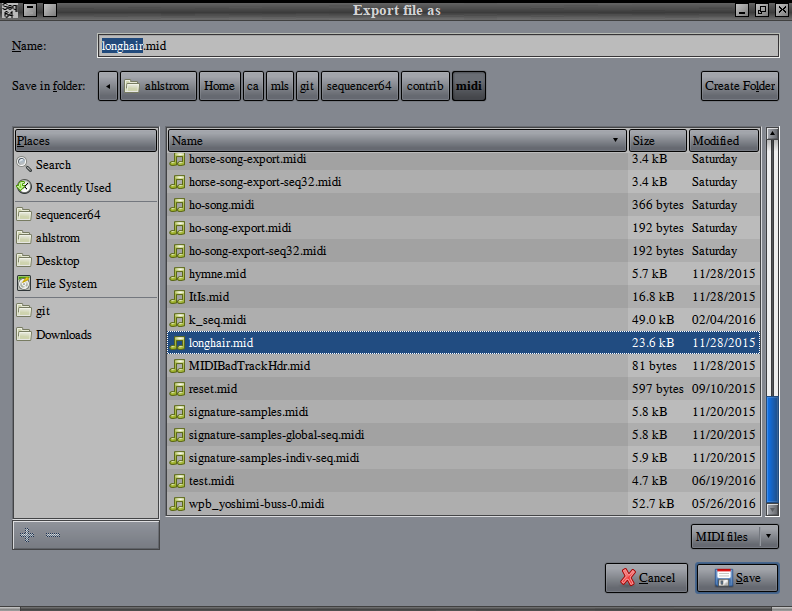
\includegraphics[scale=0.65]{menu/menu_file_export.png}
   \caption{File / Export Song as MIDI}
   \label{fig:seq64_menu_file_export}
\end{figure}

   If there are no exportable tracks, the following message is shown:

\begin{figure}[H]
   \centering 
   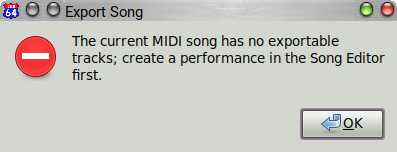
\includegraphics[scale=0.75]{menu/menu_file_unexportable.png}
   \caption{Unexportable MIDI File}
   \label{fig:seq64_menu_file_unexportable}
\end{figure}

   Once the file has been exported, it can be opened in order to see
   the results of the export.  Both the main window view and the
   song performance view will show the results of the export.

   Here is a short song, in two sets, shown in a composite view of four windows,
   showing each set and the performance layout of the tracks in the sets.

\begin{figure}[H]
   \centering 
   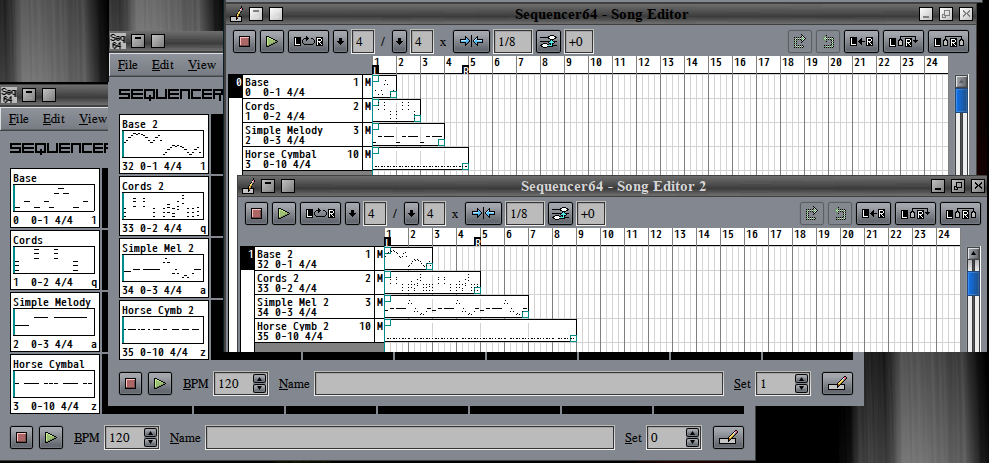
\includegraphics[scale=0.50]{export/original-song-to-export.png}
   \caption{Composite View of Exportable Song}
   \label{fig:seq64_original_song_to_export}
\end{figure}

   The left column shows the four tracks of the first set (Set 0), the next
   column shows the four tracks of the second set (Set 1), and the
   layouts of the two sets are shown in the remainder of the diagram.

   Now let's export this song, and see the result:

\begin{figure}[H]
   \centering 
   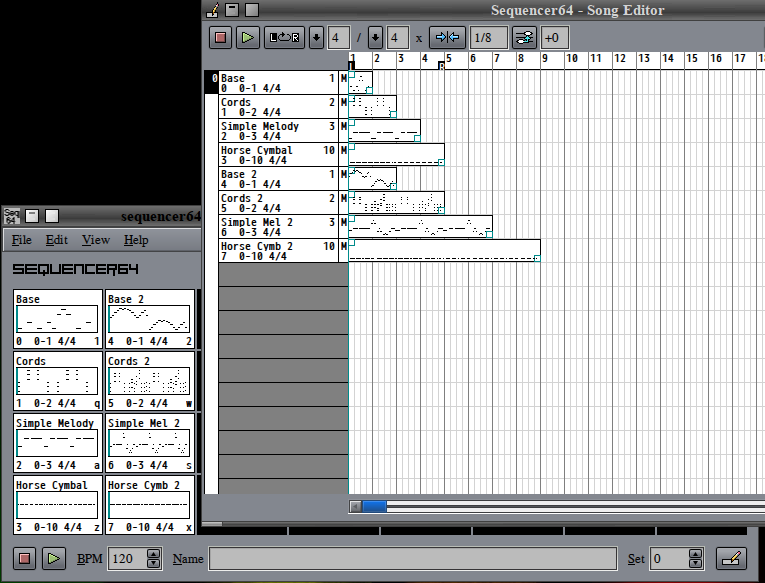
\includegraphics[scale=0.75]{export/song-exported.png}
   \caption{Composite View of Exported Song}
   \label{fig:seq64_song_exported}
\end{figure}

   Once can see that the two sets are now combined into the first set,
   and all of the track layouts (triggers) have been exported.
   Had there been gaps in layouts or repeats of layouts in the song/performance
   data, these would have been reflected in the triggers.
   Much more complex examples are, of course, possible.

\subsubsection{Menu / File / Options}
\label{subsubsec:seq64_menu_file_options}

   The \textbf{Options} menu item provides a number of settings in one
   tabbed dialog, shown in the figures that follow.
   This dialog allows one to select which sequence gets the MIDI
   clock, which incoming MIDI events control the sequencer, what keys are
   mapped to functions, how the mouse works, and some JACK parameters.

   Note that there is now an extra tab-page for \textbf{Ext Keys}.
   It is not shown in some of the screenshots; we are too lazy to re-do those
   screenshot just to show the new tab.

\begin{figure}[H]
   \centering 
   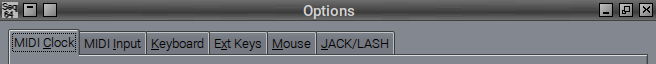
\includegraphics[scale=0.75]{menu/options-tab-0-9-18.png}
   \caption{File / Options Tabs for Version 0.9.18+}
   \label{fig:seq64_options_tab_0_9_18}
\end{figure}

\paragraph{Menu / File / Options / MIDI Clock}
\label{paragraph:seq64_menu_file_options_midi_clock}

   The \textbf{MIDI Clock} tab provides a way to send the MIDI clock to one
   or more of the \textsl{Sequencer64} output busses.
   It is used to configure to what busses the MIDI clock gets dumped.
   It also shows the devices that can play music.
   The items that appear in this tab depend on four things:

   \begin{itemize}
      \item What MIDI devices are connected to the computer.  For example,
         MIDI controllers, USB MIDI cables, and other devices will add MIDI
         output devices (ports) to the system.
      \item What MIDI software devices are running on the computer.
         For example, running MIDI software synthesizers such as
         \textsl{Timidity} and \textsl{Yoshimi} will add extra output devices
         (playback ports) to a system.
      \item The setting of the "manual ALSA ports" option,
         \texttt{--manual-alsa-ports} command-line option or the
         \texttt{[manual-alsa-ports]} section of the
         \texttt{sequencer64.rc} configuration file, as described in
         \sectionref{subsec:seq64_rc_file_other_midi}
      \item The setting of the \textsl{Sequencer64}-specific
         "reveal ALSA ports" option,
         \texttt{--reveal-alsa-ports} command-line option or the
         \texttt{[reveal-alsa-ports]} section of the
         \texttt{sequencer64.rc} configuration file, as described in
         \sectionref{subsec:seq64_rc_file_other_midi}
   \end{itemize}

   For the current discussion, a USB MIDI cable was plugged into the system,
   and the \textsl{Timidity} and \textsl{Yoshimi} (in ALSA mode) software
   synthesizers were running.  \textsl{Sequencer64} was also running, of
   course, with the option of "manual ALSA ports" (\texttt{-m} or
   \texttt{--manual-alsa-ports}) and ALSA (\texttt{-A} or
   \texttt{--alsa} turned on.
   Here are the devices shown by the ALSA MIDI playback
   command-line application:

   \begin{verbatim}
      $ aplaymidi -l
       Port    Client name                      Port name
       14:0    Midi Through                     Midi Through Port-0
       24:0    E-MU XMidi1X1 Tab                E-MU XMidi1X1 Tab MIDI 1
      128:0    TiMidity                         TiMidity port 0
      128:1    TiMidity                         TiMidity port 1
      128:2    TiMidity                         TiMidity port 2
      128:3    TiMidity                         TiMidity port 3
      129:16   sequencer64                      sequencer64 in
   \end{verbatim}

%  (For some reason, the \textsl{Yoshimi} input port is not showing up
%  in the output of \texttt{aplaymidi}, though, as shown in
%  \figureref{fig:seq64_midi_clock_4_devices_manual_0},
%  \textsl{Sequencer64} sees it on port 7.  Perhaps that application is not
%  providing a good ALSA device name.)

   Turning to \figureref{fig:seq64_midi_clock_4_devices_manual_1},
   note the 16 devices provided by
   \textsl{Sequencer64}.  Also note that its first value is 1, not 0, due to
   the MIDI Thru port occupying slot 0.
   This figure shows the result with the "manual ALSA option" turned on.
   But remember that, now this option also applies to the native JACK MIDI
   version of \textsl{Sequencer64}, which has an executable named
   \texttt{seq64}.

\begin{figure}[H]
   \centering 
%  \includegraphics[scale=0.75]{menu/midi-clock-4-devices-manual-1.png}
%  \includegraphics[scale=0.75]{new/midi-clock-4-devices-manual-1.png}
   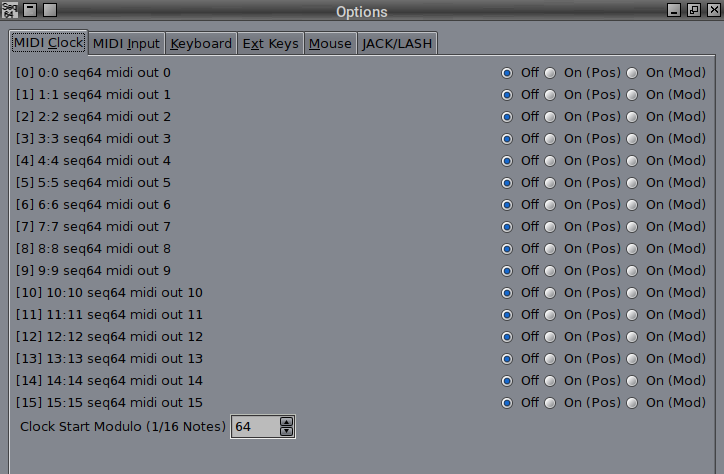
\includegraphics[scale=0.75]{jack/jack-nano-yosh-manual-clock-seq64.png}
   \caption{MIDI Clock, Manual Option On}
   \label{fig:seq64_midi_clock_4_devices_manual_1}
\end{figure}

   It basically shows the 16 MIDI output busses that \textsl{Sequencer64} can
   drive.  One would have to use a JACK or ALSA MIDI connection application to
   put a device on each of those outputs.  The fact that the the buss names can
   start with different numbers, depending on the system setup, can complicate
   the playing of MIDI in this manner.  Also, the "user" configuration file can
   change the names of the ports, causing further confusion.
   The following elements are present in this dialog:

   \begin{enumber}
      \item \textbf{Index Number}
      \item \textbf{Client Number}
      \item \textbf{Port Number}
      \item \textbf{Buss Name}
      \item \textbf{Off}
      \item \textbf{On (Pos)}
      \item \textbf{On (Mod)}
      \item \textbf{Clock Start Modulo}
   \end{enumber}

   \setcounter{ItemCounter}{0}      % Reset the ItemCounter for this list.

   \itempar{Index Number}{midi clock!index number}
   \index{index number}
   The number in square brackets is simply an ordinal indicating the position
   of the output buss in the list of busses.
   It can be used with the \texttt{--bus} option to redirect all output to that
   one buss.

   \itempar{Client Number}{midi clock!client number}
   \index{client number}
   The number that precedes the colon is the "client number".
   It is useful mainly in ALSA, where clients can have numbers like "14",
   "128", "129", etc.  For native JACK mode, it just matches the index number.

   \itempar{Port Number}{midi clock!port number}
   \index{port number}
   The number that follows the colon is the "port number".
   It is useful mainly in ALSA.
   For native JACK mode, it just matches the index number.

   \itempar{Buss Name}{midi clock!buss name}
   \index{port name}
   \index{midi clock!port name}
   These labels indicate the output busses (ports) of \textsl{Sequencer64}.
   They range from \textbf{[1] sequencer64 1} to \textbf{[16] sequencer64 16}
   in the legacy application, \texttt{sequencer64}.
   They range from \textbf{[1] seq64 1} to \textbf{[16] seq64 16}.
   in the native JACK application, \texttt{seq64}.

   \itempar{Off}{midi clock!off}
   This setting disables the MIDI clock for the given output buss.
   However, note that MIDI output can still be sent to those ports, and
   each port that has a device connected to it will play music.

   For feeding \textsl{Yoshimi} (running in ALSA mode)
   with MIDI data, we found that this
   setting is the one that must be made in order for \textsl{Yoshimi} to
   produce a sound.

   \itempar{On (Pos)}{midi clock!on (pos)}
   The MIDI clock will be sent to this buss.
   MIDI Song Position and MIDI Continue will be sent if playback is starting
   at greater than tick 0 in Song mode.  Otherwise, MIDI Start will be sent.

   \itempar{On (Mod)}{midi clock!on (mod)}
   The MIDI clock will be sent to this buss.
   MIDI Start will be sent and clocking will begin
   once the Song Position has reached the start modulo of the specified size
   (see the next item's description).
   This setting is used for gear that does not respond to Song Position.

   \itempar{Clock Start Modulo}{midi clock!clock start modulo}
   Clock Start Modulo (1/16 Notes).
   This value starts at 1 and ranges on upward to 16384.
   It  defaults to 64.
   It is used by the \textbf{On (Mod)} setting discussed above.
   It is the \texttt{[midi-clock-mod-ticks]} option in the \textsl{Sequencer64}
   "rc" file as described in
   \sectionref{subsec:seq64_rc_file_other_midi}.

\begin{figure}[H]
   \centering 
%  \includegraphics[scale=0.75]{menu/midi-clock-4-devices-manual-0.png}
   \includegraphics[scale=0.75]{new/midi-clock-4-devices-manual-0.png}
   \caption{MIDI Clock, Manual Option Off (ALSA View)}
   \label{fig:seq64_midi_clock_4_devices_manual_0}
\end{figure}

   As shown by the figure above, with the "manual ALSA option" turned off,
   all of the devices that can be driven by MIDI output are shown,
   including the MIDI Thru port, the MIDI port on the
   \textsl{E-MU XMidi1x1} USB cable,
   the four ports provided by \textsl{Timidity}, and the unlabelled
   port provided by the \textsl{Yoshimi} synthesizer running in ALSA mode.
   (However, \texttt{seq64} does show the name "yoshimi" as the client name.)
   One could theoretically play music through 6 or 7 devices using
   \textsl{Sequencer64} with this setup.

   See \sectionref{subsec:seq64_jack_native_midi}
   for a lot more information about native JACK support, and examples of JACK
   MIDI ports and connections.

   \textbf{TODO:}
   \index{todo!manual alsa gui option}
   There is currently no user-interface item corresponding to the "manual ALSA"
   command-line and "rc" configuration file option.
   We also want to rename this option to simply "manual" in the near future.

\paragraph{Menu / File / Options / MIDI Input}
\label{paragraph:seq64_menu_file_options_midi_input}

   To allow \textsl{Sequencer64} to record MIDI from MIDI devices such as
   controllers and keyboards, the output of the ALSA MIDI recording
   command-line application is relevant:

   \begin{verbatim}
      $ arecordmidi -l
       Port    Client name                      Port name
       14:0    Midi Through                     Midi Through Port-0
       24:0    USB2.0-MIDI                      USB2.0-MIDI MIDI 1
      129:0    sequencer64                      [1] sequencer64 1
      129:1    sequencer64                      [2] sequencer64 2
      129:2    sequencer64                      [3] sequencer64 3
       . . .   . . .                               . . .
      129:15   sequencer64                      [16] sequencer64 16
   \end{verbatim}

   We see that we can record MIDI from the MIDI Thru port, from the USB MIDI
   cable, and MIDI from any of the 16 output ports provided by the manual ALSA
   port mode of \textsl{Sequencer64}.

   If the "manual ALSA ports" option is turned on,
   then the only item in the \textbf{MIDI Input} tab is the single MIDI input
   buss provided by \textsl{Sequencer64}:  \textbf{[0] sequencer64 0}, or, since
   the MIDI Thru port takes slot 0, \textbf{[1] sequencer64 1}.

\begin{figure}[H]
   \centering 
%  \includegraphics[scale=0.75]{menu/midi-input-4-devices-manual-1.png}
   \includegraphics[scale=0.75]{new/midi-input-4-devices-manual-1.png}
   \caption{MIDI Input, Manual Ports On (Condensed View)}
   \label{fig:seq64_midi_input_4_devices_manual_1}
\end{figure}

   This item, if checked, allows \textsl{Sequencer64} to be used to record MIDI
   information from another source (which must be connected to this port by
   another application), or pass it through to the output busses
   that are configured to allow pass-through
   (in the Pattern Editor, as discussed in 
   \sectionref{subsec:seq64_pattern_editor_bottom}.)

   \textbf{Warning:}
   \index{warnings!usr config}
   \index{usr config}
   If the 
   \texttt{[user-midi-bus-definitions]} value in the "user" configuration file
   is non-zero, and the
   corresponding number of
   \texttt{[user-midi-bus-N]} settings are provided, then
   the list of existing hardware will be ignored, and those values will be
   shown instead.
   (This feature can be overridden with the
   \texttt{--reveal-alsa-ports} (\texttt{-r}) option.)

%  New in \textsl{Sequencer64} is the option to record MIDI input into
%  more than one pattern based on the MIDI channel, as discussed below.

   If the "manual ALSA ports" option is turned off, then
   the input ports from the system are shown:

\begin{figure}[H]
   \centering 
%  \includegraphics[scale=0.75]{menu/midi-input-4-devices-manual-0.png}
   \includegraphics[scale=0.75]{new/midi-input-4-devices-manual-0.png}
   \caption{MIDI Input, Manual ALSA Ports Off (Condensed View)}
   \label{fig:seq64_midi_input_4_devices_manual_0}
\end{figure}

   For example, one could check input \#1 to have \textsl{Sequencer64} record
   MIDI from an old-fashioned MIDI keyboard that is connected to another
   USB MIDI cable (the \textsl{E-MU Xmidi}).  If the keyboard didn't have a
   sound generator, one would also want \textsl{Sequencer64} to pass this MIDI
   on to a sound generator, such as a software or hardware synthesizer attached
   to one of the ports shown in
   \figureref{fig:seq64_midi_clock_4_devices_manual_0}.

   \textbf{Warning:}
   \index{warnings!usr config}
   \index{usr config}
   Again, note that the "user" configuration file can override what is actually
   displayed as hardware.  If you define these sections, they should match your
   hardware exactly, and your hardware should not change from session to
   session.

   Note the two sections of this configuration page:

   \index{input buses}
   \textbf{Input Buses} delineates the MIDI input devices as noted above.
   \index{input options}
   \textbf{Input Options} adds further refinements to MIDI input.  The current 
   option present

   \index{input by channel}
   \textbf{Record input into sequence according to channel},
   is a new (and \textsl{untested}) feature ported from \textsl{Seq32}.
   When enabled, MIDI input with multiple channels is distributed to
   each sequence according to what MIDI channel the sequence is set to.
   When disabled, the legacy recording behavior dumps all data into the current
   sequence, regardless of channel.

\paragraph{Menu / File / Options / Keyboard }
\label{paragraph:seq64_menu_file_options_keyboard}

   \textsl{Seq24} allows extensive use of
   keyboard shortcuts to make operations go faster than when using a mouse,
   and \textsl{Sequencer64} extends that tradition.
   The \textbf{Keyboard} tab allows for the configuration of these keyboard
   shortcuts.

   \textbf{Warning:}
   \index{keys!gotchas}
   There are a number of "gotchas" to be aware of when assigning keys to the
   fields in the \textbf{Keyboard} tab:

   \begin{itemize}
      \item Whenever one of the text fields in this dialog has the focus (and
         that is usually the case), then any keystroke, including keys like
         Ctrl, Alt, and Super (Mod4 or Windows key), can alter the value of a
         field to that of the keystroke.  This change is very easy to do
         accidentally!  \textsf{Use the mouse} to move this window and to click
         its \textbf{OK} button!
      \item Some of the keys traditionally used (or used by default) for
         control have been adapted for other uses.  One example is
         \texttt{Ctrl-L}, which brings up the learn mode that can be started
         using the "L" button.
      \item \textsl{Sequencer64} has appropriated the
         \index{keys!shift} Shift key so that it
         modifies a click on a pattern so that all of the other patterns are
         \textsl{toggled}.  Therefore, using characters that require the Shift
         key while clicking, such as \texttt{\{} and \texttt{\}}, when used
         to set the \textbf{Replace} function, becomes surprising.
         Instead, look to the remaining keys: \texttt{F11}, \texttt{F12},
         and the "keypad" keys if more options are wanted.  Be sure to
         look at the \textbf{Ext Keys} tab to see what other keys are in use.
   \end{itemize}

\begin{figure}[H]
   \centering 
%  \includegraphics[scale=0.75]{menu/menu_file_options_keyboard.png}
%  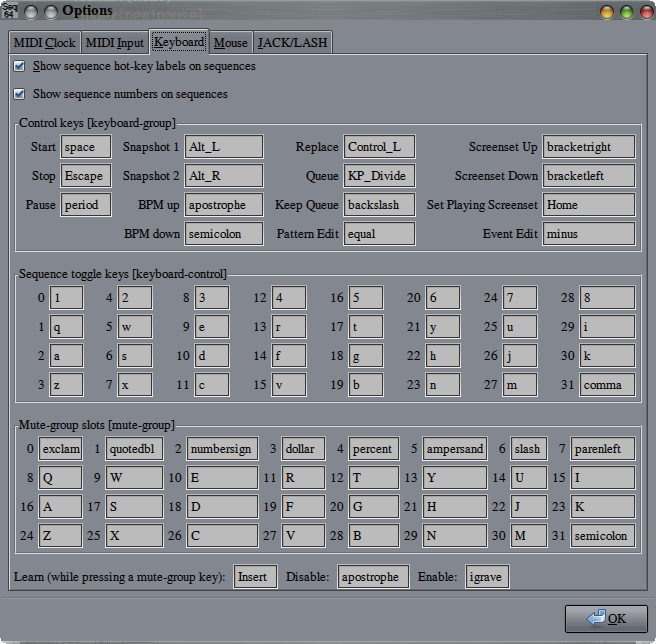
\includegraphics[scale=0.75]{menu/menu_file_options_keyboard-0_9_12.png}
   \includegraphics[scale=0.75]{new/menu_file_options_keyboard.png}
   \caption{File / Options / Keyboard (Condensed View)}
   \label{fig:seq64_menu_file_options_keyboard}
\end{figure}

   Note the new \textbf{Ext Keys} tab is not shown in this figure.
   We won't attempt to cover every user-interface item in this busy
   dialog, just the categories.  Some items are discussed in other parts of
   this manual.

   \textbf{New:}
   \index{new!pause}
   \index{pause}
   Also, if the application has been built with the pause option, an
   additional key definition is shown for the Pause key.

   By default, the Pause key is the period (".").  An old version of
   the "rc" file is automatically fixed to include this new option.
   (The pause feature can be removed by rebuilding the application
   after configuring with the \texttt{--disable-pause} option.)

% \begin{figure}[H]
%    \centering 
%    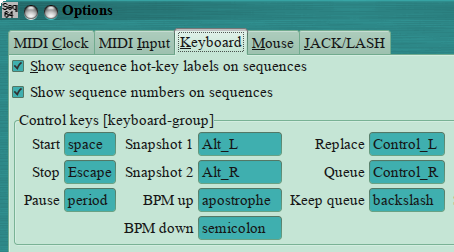
\includegraphics[scale=0.75]{new/keyboard-options-0_9_10_1.png}
%    \caption{File / Options / Keyboard, with Pause}
%    \label{fig:seq64_menu_file_options_keyboard_pause}
% \end{figure}

   \textbf{New:}
   \index{new!pattern edit}
   \index{pattern edit}
   \index{new!event edit}
   \index{event edit}
   With version 0.9.12, we add a new feature as we try to achieve the goal of
   being able to edit a pattern using only the keyboard.
   \textsl{Sequencer64} now supports two modifier keys.
   The first modifier key causes the usual pattern-toggle key (hot-key) for a
   given slot to instead bring up the pattern editor.  By default, this key is
   the equals ("=") key.  The second modifier key causes the usual
   pattern-toggle key (hot-key) for a given slot to instead bring up the event
   editor.  By default, this key is the minus ("-") key.
   These keys are currently hard-wired, but we'll make them configurable
   eventually.
%  As with the other
%  keys, these keys can be reconfigured to a different set of keys in the
%  \textbf{File / Options / Keyboard} page.

   To continue with a listing of the keyboard options:

   \begin{enumber}
      \item \textbf{Show sequence hot-key labels on sequences}
      \item \textbf{Show sequence numbers on sequences}
      \item \textbf{Control keys [keyboard-group]}
      \item \textbf{Sequence toggle keys [keyboard-control]}
      \item \textbf{Mute-group slots [mute-group]}
      \item \textbf{Learn}
      \item \textbf{Disable}
      \item \textbf{Enable}
   \end{enumber}

   \setcounter{ItemCounter}{0}      % Reset the ItemCounter for this list.

   \itempar{Show key labels on sequence}{keyboard!show labels}
   This item, if enabled, shows the key labels in the lower-right corner of
   each loop/pattern in the Patterns window (the main window).  This feature is
   useful for live playback and control of a song.
   Note that this option is also available in the "rc" configuration file.

   \itempar{Show sequence numbers on sequence}{keyboard!sequence numbers}
   \textbf{New:}
   \index{new!sequence numbers}
   If this option is turned on, the
   empty slots in the Patterns window show the prospective sequence number.
   See the following figure for one look of this feature.

\begin{figure}[H]
   \centering 
%  \includegraphics[scale=0.75]{pattern-window-with-numbering.png}
   \includegraphics[scale=0.75]{new/pattern-window-with-numbering.png}
   \caption{Pattern Window with Numbering}
   \label{fig:seq64_build_with_numbering}
\end{figure}

   If one doesn't like it, turn off the option in the "rc" configuration file,
   or try other grid options in the "user" configuration file.
   Also note that the option also changes the visibility of sequence numbers
   in active sequences and in the Song Editor's names column.

   \itempar{Control keys}{keyboard!control keys}
   This block of fields in the \textbf{Options / Keyboard} tab
   provides shortcut keys for many operations of
   \textsl{Sequencer64}.

   \begin{enumber}
      \item \textbf{Start}.
         Key: \index{keys!space} \textbf{space}.
      \item \textbf{Stop}.
         Key: \index{keys!esc} \textbf{Escape}.
      \item \textbf{Pause}. (new)
         Key: \index{keys!period} \textbf{period}.
      \item \textbf{Snapshot 1}.
         Key: \index{keys!alt-l} \textbf{Alt\_L}.
      \item \textbf{Snapshot 2}.
         Key: \index{keys!alt-r} \textbf{Alt\_R}.
      \item \textbf{bpm up}.
         Key: \index{keys!apostrophe} \textbf{apostrophe}.
      \item \textbf{bpm down}.
         Key: \index{keys!semicolon} \textbf{semicolon}.
      \item \textbf{Replace}.
         Key: \index{keys!ctrl-l} \textbf{Control\_L}.
      \item \textbf{Queue}.
         Key: \index{keys!ctrl-r} \textbf{Control\_R}.
      \item \textbf{Keep queue}.
         Key: \index{keys!backslash} \textbf{backslash}.
      \item \textbf{Screenset down}.
         Key: \index{keys![} \textbf{bracketleft}.
      \item \textbf{Screenset up}.
         Key: \index{keys!]} \textbf{bracketright}.
      \item \textbf{Set playing screenset}.
         Key: \index{keys!home} \textbf{Home}.
   \end{enumber}

   Note that some of the keys have positional mnemonic value.  For example,
   for BPM control, the semicolon is at the left (down), and the apostrophe
   is at the right (up).
   Also note that the keys definable in this tab are only a subset of the
   various keys that can be used, especially keys used with the
   \texttt{Ctrl} key or other modifier keys.

   \index{snapshot}
   \index{keys!snapshot}
   A \textsl{snapshot} is a briefly preserved state of the patterns.
   One can press a snapshot key, change the state of the patterns for live
   playback, and then release the snapshot key to revert to the state when
   the snapshot key was first pressed.

   \index{queue}
   \index{keys!queue}
   To \textsl{queue}
   a pattern means to ready it for playback upon the next repeat
   of a pattern.  A pattern can be armed immediately, or it can be queued to
   play back the next time the pattern starts.
   A pattern can be queued by holding the queue key (defined in
   \textbf{File / Options / Keyboard / queue}) and pressing a pattern-slot
   shortcut key.  Instead of the pattern turning on immediately, it turns on at
   the next repeat of the pattern.

   \index{keep queue}
   \index{keys!keep queue}
   \index{queue!keep}
   The \textsl{keep queue}
   functionality allows the queue to be held without holding
   down the queue button the whole time.  First, press the keep-queue key
   (defined in \textbf{File / Options / Keyboard / Keep queue}).  Now, hitting
   any of the shortcut keys, no matter how many, sets up the corresponding
   pattern slot to be queued.  This mode is disabled by hitting the
   "queue" key (any currently active queues remain active until finished).

   \itempar{Sequence toggle keys}{keyboard!sequence toggle keys}
   Each of these keys toggles the playing/muting of one of the 32
   loop/pattern boxes.  These keys are layed out logically on the keyboard,
   and can also be shown in each loop/pattern box.  No need to list them all
   here!  Please note that we often call them "shortcut keys" where the context
   makes it clear that they apply to the armed/unarmed state of a pattern.
   Sometimes they are called "hot keys".

   \itempar{Mute-group slots}{keyboard!mute-group slots}
   Each of these keys operates on the mute-grouping of one of the 32
   loop/pattern boxes.  These keys are layed out logically on the keyboard,
   and can also be shown in each loop/pattern box.  No need to list them all
   here!

   \index{mute-group}
   One thing we need to explain is just what mute-grouping
   means functionally.

   \textsl{Mute groups} are shortcuts to play a defined group of patterns
   on the current set, while stopping other patterns from the current set, and
   all patters from other sets.

   To define the group of patterns for one mute group, press and hold the Learn
   key (the \texttt{Insert} key by default, but see the current configuration)
   and, simultaneously, press one of the mute group keys: \textsl{Sequencer64}
   will save the currently-playing pattern slots into the corresponding mute
   group.  Note that the default mute group keys need the \texttt{Shift}
   modifier, but one does not need the \texttt{Shift} key while pressing
   \texttt{Insert} to learn the group, only to trigger it (\textsl{Sequencer64}
   will automatically assign the corresponding key with \texttt{Shift}
   activated).

   Group-mute can be globally enabled or disabled (with default keys apostrophe
   \texttt{'} \index{grave} \index{igrave} and igrave or grave \texttt{`}).
   So make sure it is enabled before trying to use it.

   \itempar{Learn}{keyboard!learn}
   \index{group!learn}
   Learn (while pressing a mute-group key).
   This items sets the key used to initiate a learn mode.
   It is the \textbf{Insert} key by default.
   \index{auto-shift}
   \index{group-learn!auto-shift}
   When in group-learn mode, the \texttt{Shift} key cannot be hit, so the
   group-learn mode automatically converts the keys to their shifted versions.
   \index{shift-lock}
   \index{group-learn!shift-lock}
   This feature known as \textsl{shift-lock} or \textsl{auto-shift}.
   It is new to \textsl{Sequencer64}.

   \itempar{Disable}{keyboard!disable}
   \index{keys!apostrophe}
   It is the \textbf{apostrophe} key by default.
   \index{group!off}
   \index{keyboard!group off}
   This key is the \textsl{group off} key.

   \itempar{Enable}{keyboard!enable}
   \index{keyboard!igrave}
   It is the \textbf{igrave} (back-tick) key by default.
   \index{group!on}
   \index{keyboard!group on}
   This key is the \textsl{group on} key.

\paragraph{Menu / File / Options / Ext Keys }
\label{paragraph:seq64_menu_file_options_ext_keys}

   A number of additional functions have been added to \textsl{Sequencer64},
   and keystrokes have been provided for those new functions, in the
   \textbf{Ext Keys} page.

\begin{figure}[H]
   \centering 
   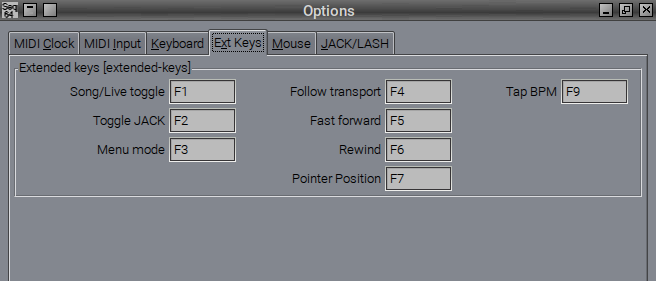
\includegraphics[scale=0.75]{menu/menu_file_options_ext_keys_condensed.png}
   \caption{File / Options / Ext Keys (Condensed View)}
   \label{fig:seq64_menu_file_options_ext_keys}
\end{figure}

% Currently there is only one block of fields.  New blocks should also be
% marked by "itempar".

   \itempar{Ext Keys}{keyboard!extended keys}
   This block of fields in the \textbf{Options / Ext Keys} tab
   provides shortcut keys for more operations of \textsl{Sequencer64}, many of
   them ported from \textsl{Seq32}.
   The default keys are shown.

   \begin{enumber}
      \item \textbf{Song/Live toggle}.
         Key: \index{keys!F1} \textbf{F1}.
      \item \textbf{Toggle JACK}.
         Key: \index{keys!F2} \textbf{F2}.
      \item \textbf{Menu mode}.
         Key: \index{keys!F3} \textbf{F3}.
      \item \textbf{Follow transport}.
         Key: \index{keys!F4} \textbf{F4}.
      \item \textbf{Fast forward}.
         Key: \index{keys!F5} \textbf{F5}.
      \item \textbf{Rewind}.
         Key: \index{keys!F6} \textbf{F6}.
      \item \textbf{Pointer Position}.
         Key: \index{keys!F7} \textbf{F7}.
      \item \textbf{Toggle mutes}.
         Key: \index{keys!F8} \textbf{F8}.
      \item \textbf{Tap BPM}.
         Key: \index{keys!F9} \textbf{F9}.
   \end{enumber}

   Most of these extended keys implement operations performed with button
   presses.  However, some of the new keystrokes do not have a corresponding
   button (yet).  Also, we still need to clarify the meaning of some of the new
   functions.

   These values are saved as the \texttt{[extended-keys]} section of the "rc"
   configuration file.  However, not all builds of \textsl{Sequencer64} will
   support the new keys.  Some of the new features can be enabled or disabled
   during the build-configure step, and one's favorite distro may decide to
   disable some features.  In this case, although the values will still be
   stored in the "rc" file, they will be disabled in this tab:

\begin{figure}[H]
   \centering 
   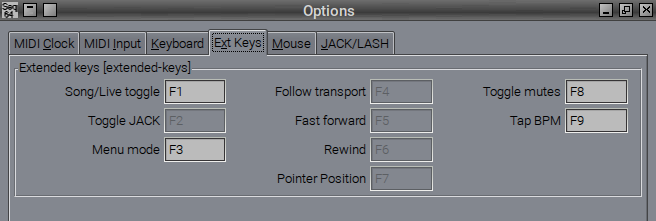
\includegraphics[scale=0.75]{menu/menu_file_options_ext_keys_disabled.png}
   \caption{File / Options / Ext Keys (Disabled)}
   \label{fig:seq64_menu_file_options_ext_keys_disabled}
\end{figure}

   \index{song mode}
   Note the \textbf{Song/Live toggle} key.
   The \textsl{song mode} normally is in effect only when playback is started
   from the \textbf{Song Editor}.  Now this mode can be used from any
   window, if enabled by pressing this key.  There is also
   a button in the main window for this function, which shows the current state
   of this flag.  Note that this flag is also stored in the "rc" configuration
   file, as well as this hotkey value, which defaults to \texttt{F1}.

   \index{toggle JACK}
   \index{JACK toggle}
   The \textsl{JACK mode} is normally set via the
   \textbf{File / Options / JACK / JACK Connect} or 
   \textbf{JACK Disconnect} buttons.
   But, if \textsl{Sequencer64} is built for using the \textsl{Seq32} JACK
   support, then this keystroke will toggle between JACK connect and JACK
   disconnect.
   Note that, with this kind of build, the \textbf{Song Editor} will also have
   a \textbf{JACK} button.
   The hotkey for this function defaults to \texttt{F2}.

   \index{menu mode}
   The \textsl{menu mode} simply indicates if the main menu of the
   main window is accessible or not.  It will be disabled in playback
   so that more hotkeys can be used without triggering menu function.
   It can also be disabled by the user; the default hotkey is \texttt{F3}.
   Here is Stazed's explanation of the feature, mildly edited:

   \begin{quotation}
      \textsl{"why disabling is needed when playing"}
      The original seq24 had numerous conflicts between the menu key binding
      and the default seq24 key binding for the mainwind sequence triggers.
      For example: Ctrl-q (quits the program without prompt). If you place a
      sequence in the default 'q' slot, you cannot use it with Ctrl-l or Ctrl-r
      (default replace or queue) because the menu grabs the keys. Same goes for
      the Alt-l or Alt-r (default snapshot 1 or 2). Try same as above with
      Alt-f, Alt-v, Alt-h, Ctrl-n, Ctrl-o...  etc. So I just shut off all the
      menus by default when playing because it seems that they should not be
      needed then... especially in a live performance.

      \textsl{"why a button?"}
      On occasion I wanted to use the mainwnd key binding when stopped to set
      the sequences to be ready before starting. It's also a sort of safety
      feature as well, just toggle the menus off before going live so that you
      don't hit Ctrl-q, Ctrl-n etc. forgetting things are not playing....
   \end{quotation}

   \index{follow transport}
   The \textsl{follow transport} functionality is a feature ported
   from \textsl{Seq32}.  We'll have more of a description of it later.
   The default key is \texttt{F4}.

   \index{fast forward}
   The \textsl{fast forward} functionality is a feature ported
   from \textsl{Seq32}.
   Basically, while this key is held, the song pointer will fast-forward
   through the song.
   The default key is \texttt{F5}.
   This feature does not (yet) have a corresponding button.
   This feature also requires that the \textsl{Seq32} transport option be
   enabled at build time.

   \index{rewind}
   The \textsl{rewind} functionality is a feature ported
   from \textsl{Seq32}.
   The default key is \texttt{F6}.
   Basically, while this key is held, the song pointer will rewind in
   the song.
   This feature does not (yet) have a corresponding button.
   This feature also requires that the \textsl{Seq32} transport option be
   enabled at build time.

   Note that, since these keys are use only in the Song Editor,
   the \textsl{seq32} keys \texttt{f} and \texttt{r} keys could be
   used as well.  Be sure not to use the following keys, which are already
   hardwired for other functions in the Song Editor:

   \begin{itemize}
      \item \texttt{p}.  Paint mode.
      \item \texttt{x}.  Escape paint mode.
   \end{itemize}


   \index{pointer position}
   The \textsl{pointer position} functionality is a feature ported
   from \textsl{Seq32}.
   The default key is \texttt{F7}.
   Basically, when this key is pressed, the song pointer will move to the
   current position of the mouse, snapped.
   This feature does not have a corresponding button.
   This feature also requires that the \textsl{Seq32} transport option be
   enabled at build time, which is the case if the \textsl{Seq32} JACK build
   option is selected (and now it is the default).

   \index{toggle mutes}
   The \textsl{toggle mutes} function toggles the mute status of every
   pattern on every screen-set.  It corresponds to the
   \textbf{Edit / Toggle mute all tracks} or the 
   \textbf{Song / Toggle All Tracks}
   menu entries.  There is also a button in the main window for this function,
   which shows the current state of this flag.  Note that this
   hotkey value is stored in the "rc" configuration file, and
   defaults to \texttt{F8}.

   \index{tap bpm}
   The \textsl{tap bpm} function allows the user to "tap" in time with some
   other music, and see the tap sequence translated into beats/minute (BPM).
   There is also a button for this function.
   After 5 seconds, this feature resets automatically, so the user can try
   again if not satisfied.  At least two clicks are needed for this
   functionality to work.

\paragraph{Menu / File / Options / Mouse }
\label{paragraph:seq64_menu_file_options_mouse}

   This item selects the mouse-interaction method.

\begin{figure}[H]
   \centering 
   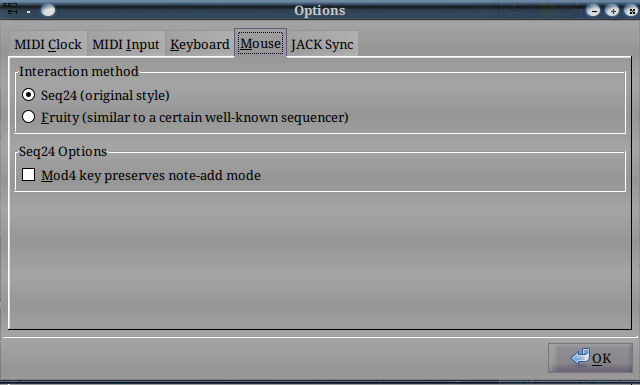
\includegraphics[scale=0.75]{menu/menu_file_options_mouse_condensed.png}
   \caption{File / Options / Mouse (Condensed View)}
   \label{fig:seq64_menu_file_options_mouse}
\end{figure}

   \index{interaction method}
   \index{mouse interaction}
   \textbf{Interaction Method}

   The default mouse interaction method is \textbf{Seq24 (original style)}.
   The alternate mouse interaction method is \textbf{Fruity (similar to a
   certain well known sequencer)}.

   \index{mouse!fruity}
   The alternate method is presumably that of the \textsl{Fruity Loops}
   (now \textsl{FL Studio}) sequencer.  The fruity mode seems to involve the
   following (based on scanning the source code):

   \begin{itemize}
      \item \textbf{Left-click left side}.
         Begin a grow/shrink operation for the left side.
      \item \textbf{Left-click right side}.
         Begin a grow/shrink operation for the right side.
      \item \textbf{Left-click middle}.
         Move the object.
      \item \textbf{Left-click}.
         Add an event if nothing selected.
      \item \textbf{Middle-click}.
         Split the note?
   \end{itemize}

   The \textsl{Seq24} "original style" is pretty much as expected for basic
   actions such as selecting and moving notes using the left mouse button.
   Drawing a note or event is a bit different, in the one must first
   \textsl{click and hold} the right mouse button, and then
   \textsl{click and drag} the right mouse button to insert notes,
   Notes are inserted to be at the current length and grid-snap values for
   the sequence editor for as long as the left button is pressed.
   Notes are inserted only up to the boundary of the sequence length.
   And, once notes are inserted, moving the mouse with the left button still
   held down simply moves the notes to the new note value of the mouse.

   If one releases the left button, then presses and holds it again,
   more notes will be added in the same way.
   This is strange, but it is a powerful way to layer notes into a short
   sequence.
   We call it the \index{draw mode} \index{mode!draw } "draw mode" or
   \index{paint mode} \index{mode!paint } "paint mode".

   Note that drawing/painting can also be done while the sequence is playing,
   and notes will be added to be played the next time the progress bar crosses
   them.

   \index{sequencer64 options}
   \textbf{Sequencer64 Options}

   This section currently contains a couple of new options.

   \index{keys!Mod4}
   \index{mouse!Mod4}
   \label{new_mod4_mode}
   \textbf{Mod4 key preserves add (paint) mode in song and pattern editors}

   In order to work better with certain trackpads, the
   "Seq24" mode of mouse interaction can be modified in the
   Pattern or Song editors so that the Mod4 key (Super or Windows key)
   can be pressed when releasing the right mouse button.
   This keeps the mouse in note-add mode.
   Another right-click, without pressing Mod4, will exit this mode.
   The reason for this feature is the crummy FocalTech touchpad on one of
   the author's laptops.  This trackpad seems to have only a single button,
   which the driver interprets as left or right depending where the finger
   is when it is clicked.  There's no way to click the right and left
   buttons at the same time.  There's no way to make a middle-click action.
   What a crock!

   Note that this option will not interfere with the Mod4 key being set
   in the \textbf{Keyboard} option tab, since the keys there mainly apply to
   the Patterns Panel (main window).

   \index{mouse!split mode}
   \label{new_split_mode}
   \textbf{Middle click splits song triggers at nearest snap (instead of
   halfway point)}

% Move this section to the right place and simply create a section-reference to
% it here.

   \index{paint mode}
   Another way to turn on the paint mode has been added, based on a feature
   found in a patch that someone posted about in some mailing list somewhere on
   the internet.
   To turn on the paint mode, press the
   \index{keys!p}
   \texttt{p} key while in the sequence editor.
   This is just like pressing the right mouse button, but the draw/paint mode
   sticks (as if the Mod4 mode were in force).
   To get out of the paint mode, press the
   \index{keys!x}
   \texttt{x} key while in the sequence editor.
   These keys, however, do not work (currently) while the sequence is playing.

   \index{todo:extend mouse support}
   These convenience options are limited to the
   pattern/sequence editor window and the performance editor window, and may
   need some heavier testing.  Also note that some \textsl{Sequencer64} windows
   can use the ctrl-left-click as a middle click. 
 
\paragraph{Menu / File / Options / Jack Sync and LASH}
\label{paragraph:seq64_menu_file_options_jack_sync}

   This tab sets up options for JACK synchronization, if \textsl{Sequencer64}
   was built with JACK support.  (Why wouldn't it be?)
   It now also supports native JACK MIDI.
   This tab also sets up options for using LASH session management, if
   \textsl{Sequencer64} was build with LASH support.

\begin{figure}[H]
   \centering 
%  \includegraphics[scale=0.75]{menu/menu_file_options_jack_sync.png}
%  \includegraphics[scale=0.75]{new/menu_file_options_jack_sync.png}
   \includegraphics[scale=0.75]{jack/menu_file_options_jack_sync.png}
   \caption{File / Options / JACK/LASH}
   \label{fig:seq64_menu_file_options_jack_sync}
\end{figure}

   The main sections in this dialog are:

   \begin{enumber}
      \item \textbf{JACK Transport/MIDI}
      \item \textbf{JACK Start Mode}
      \item \textbf{JACK Transport Connect and Disconnect}
      \item \textbf{LASH Options}
   \end{enumber}

   \setcounter{ItemCounter}{0}      % Reset the ItemCounter for this list.

   \itempar{Transport/MIDI}{jack sync!transport/midi}
   These settings are stored in the "rc" file settings group
   \texttt{[jack-transport]}.
   See \sectionref{subsec:seq64_rc_file_jack_transport},
   which describes this configuration option.
   This items collects the following settings:

   \begin{itemize}
      \item \textbf{Jack Transport}.
         \index{JACK!transport}
         Enables slave synchronization with JACK Transport.
         The command-line option is \texttt{--jack-transport}.
         The behavior of this mode of operation is perhaps not quite
         correct.  Even as a slave, \textsl{Sequencer64} can start and
         stop playback.
      \item \textbf{Transport Master}.
         \index{JACK!transport master}
         \textsl{Sequencer64} will attempt to serve as the JACK Master.
         The command-line option is \texttt{--jack-master}.
         \textbf{Tip}:
         \textsl{Sequencer64} generally works a little better as JACK
         master.
      \item \textbf{Master Conditional}.
         \index{JACK!master conditional}
         \textsl{Sequencer64} will fail to serve as the JACK Master if there is
         already a Master set.
         The command-line option is \texttt{--jack-master-cond}.
      \item \textbf{Native JACK MIDI}.
         \index{JACK!native midi}
         This option is for the \texttt{seq64} version of
         \textsl{Sequencer64}.
         If set, MIDI input and output occur using the new JACK MIDI interface,
         rather than using ALSA.  However, if JACK is not running on the
         system, then \texttt{seq64} will fall back to ALSA mode.
         The command-line option is \texttt{--jack-midi}.
   \end{itemize}

   Note that there are long-standing issues with the JACK support of
   \textsl{Seq24}, and \textsl{Sequencer64} currently inherits some of them,
   in spite of some bug fixes.  Generally, if one experiences issues in
   transport control, try making one of the other sequencer applications the
   JACK Master.
   If one starts \textsl{Sequencer64} in JACK mode without JACK running,
   it will take a little while for \textsl{Sequencer64} to start up, and it
   will fall back to ALSA usage.

   Finally, if one makes a change in the JACK transport settings, it is best to
   then press the \textbf{JACK Transport Disconnect} button, then the
   \textbf{JACK Transport Connect} button.  Another option is to restart
   \textsl{Sequencer64}... the settings are automatically saved when
   \textsl{Sequencer64} exits.

   \itempar{JACK Start mode}{jack sync!start mode}
   This item collects the following settings, also stored in the "rc" file
   settings group \texttt{[jack-transport]}.

   \begin{itemize}
      \item \textbf{Live Mode}.
         \index{JACK!live mode}
         \index{live mode}
         \index{non-playback mode}
         Playback will be in live mode.  Use this option to allow muting and
         unmuting of patterns.  This option might also be called "non-playback
         mode".
         The command-line option is \texttt{--jack-start-mode 0}.
      \item \textbf{Song Mode}.
         \index{JACK!song mode}
         \index{song mode}
         \index{playback mode}
         \index{performance mode}
         Playback will use only the Song Editor's data.
         The command-line option is \texttt{--jack-start-mode 1}.
   \end{itemize}

   Note that, in ALSA mode (non-JACK mode), \textsl{Sequencer64} 
   now \textsl{does} select the playback modes
   according to which window started the playback.
   We have reverted back to legacy \textsl{Seq24} behavior.

   \textsl{The main window, or pattern
   window, causes playback to be in live mode.  The user can arm and mute
   patterns in that windows, by clicking on sequences, using their hot-keys,
   and by using the group-mode and learn-mode features.
   The song editor causes playback to be in performance mode, also known as
   "playback mode", or "song mode".}
   Of course, in JACK mode,
   it selects them according to the chosen live/song mode as discussed above.

   \itempar{Connect}{jack sync!connect}
   Connect to JACK Sync.
   This button is useful to restart JACK sync when making changes to it,
   or when \textsl{Sequencer64} was started in ALSA mode.

   \itempar{Disconnect}{jack sync!disconnect}
   Disconnect from JACK Sync.
   This button is useful to stop JACK sync when making changes to it.

   \itempar{LASH Options}{lash!option}
   Currently contains only one item, which enables the usage of LASH session
   management.  Currently, \textsl{Sequencer64} needs to be restarted to
   complete the enabling or disabling of LASH support.  Like the rest of the
   options, this one is written to the "rc" configuration file.

   Finally, there is a new button (labelled \textsl{Master} in the following
   figure) in the main window to bring up directly the
   \textbf{JACK} (or \textbf{JACK/LASH}) page.

\begin{figure}[H]
   \centering 
%  \includegraphics[scale=0.75]{menu/menu_file_options_jack_sync.png}
   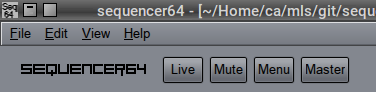
\includegraphics[scale=0.75]{new/main_master_button.png}
   \caption{JACK Connection Button}
   \label{fig:seq64_main_master_button}
\end{figure}

   This button not only brings up the JACK page, but also shows the current
   status of the MIDI connection:
   \textbf{Master} (JACK Master),
   \textbf{JACK} (JACK Slave),
   \textbf{Native} (native JACK MIDI),
   and \textbf{ALSA}.
   \index{jack page!ctrl-p}
   \index{keys!ctrl-p}
   Currently, the \texttt{Ctrl-P} will also bring up this page.

\subsection{Menu / Edit}
\label{subsec:seq64_menu_edit}

   The \textbf{Edit} menu has undergone some expansion lately.

\begin{figure}[H]
   \centering 
   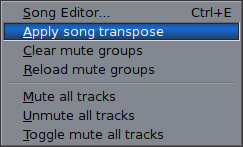
\includegraphics[scale=0.75]{new/menu_edit_0_90.png}
   \caption{Edit Menu}
   \label{fig:seq64_menu_edit_0_90}
\end{figure}

   \begin{enumber}
      \item \textbf{Song Editor...}
      \item \textbf{Apply song transpose}
      \item \textbf{Clear mute groups}
      \item \textbf{Reload mute groups}
      \item \textbf{Mute all tracks}
      \item \textbf{Unute all tracks}
      \item \textbf{Toggle mute all tracks}
   \end{enumber}

   \itempar{Song Editor}{edit!song editor}
   \index{song editor}
   This item is the same as the 
   \textbf{View / Song Editor toggle} menu entry.  It toggles the presence of
   the main song editor.

   \itempar{Apply song transpose}{edit!song transpose}
   \index{song transpose}

   Selecting this item applies the song transposition value to
   \textbf{all} sequences/patterns that are marked as transposable.
   (Normally, drum tracks are \textsl{not} transposable).
   This actively changes the note/pitch value of all note and aftertouch events
   in the pattern.

   Once the transpositions are done, the transposition value is set to 0.
   For the setting of song transpose, see
   \sectionref{sec:seq64_song_editor}, for more information.
   Also note that transpose can be enabled in the patterns panel for each
   pattern (see \sectionref{subsubsec:seq64_patterns_pattern_filled}) and
   in the sequence editor
   (see \sectionref{sec:seq64_pattern_editor}).

   \itempar{Clear mute groups}{edit!clear mute groups}
   \index{mute groups}

   A feature of \textsl{Seq24} and \textsl{Sequencer64} is that the mute groups
   are saved in both the "rc" file
   (see \sectionref{subsec:seq64_rc_file_mute_group})
   and in the "MIDI" file
   (see \sectionref{subsec:legacy_midi_format}).

   This menu entry clears them.  If the MIDI file is saved, it then has no
   mute-group information.  And then, currently, if the application is exited,
   the clear mute-group information is also saved.  We'd like to be able
   to handle the "rc" and "MIDI" mute-groups separately in the future.

   \itempar{Reload mute groups}{edit!load mute groups}
   \index{rc!mute groups}

   This menu entry reloads the mute-groups from the "rc" file.
   So, if one loads a MIDI file that has its own mute groups that one does not
   like, this command will restore one's favorite mute-grouping from the "rc"
   file.

   \itempar{Mute all tracks}{edit!mute all tracks}
   \index{mute all}

   This menu entry, available only in \textbf{Live} mode,
   immediately mutes \textsl{all} patterns in the entire song.

   \itempar{Unmute all tracks}{edit!unmute all tracks}
   \index{unmute all}

   This menu entry, available only in \textbf{Live} mode,
   immediately unmutes \textsl{all} patterns in the entire song.

   \itempar{Toggle mute all tracks}{edit!toggle all tracks}
   \index{toggle mute all}

   This option toggles the mute/armed status of \textbf{all} tracks.
   It is only available in \textbf{Live} mode, which overrides \textbf{Song}
   mode even if the Song Editor is focussed.

   \textsl{Do not confuse it with the main \textbf{Mute} button, which toggles the
   status only of the tracks that are armed and remembers them.}

\subsection{Menu / View}
\label{subsec:seq64_menu_view}

   If the "allow two perfedits" option is turned off in the "user"
   configuration file, this menu item has only one entry, \textbf{Song Editor}, 
   which is already covered by a button at the bottom of the Patterns
   window.  Selecting this item bring up the Song Editor window.
   See \figureref{fig:song_editor_window}.
   The Song Editor window can also be brought up via the
   \index{song editor!ctrl-e}
   \index{keys!ctrl-e}
   Ctrl-E key.

   If the \textbf{allow two perfedits} option is turned on in the "user"
   configuration file, this menu item has two entries, as shown in the
   following figure:

\begin{figure}[H]
   \centering 
   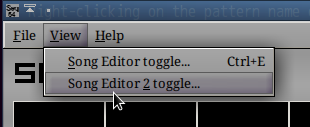
\includegraphics[scale=0.75]{menu/menu_view-dual-song-editors.png}
   \caption{Dual Song Editor Entries in View Menu}
   \label{fig:seq64_menu_view_song_editors}
\end{figure}

   Note that only the first Song Editor has a user-interface button and
   a hot-key.  Also note that there can be issues bringing up the second
   song-editor with the hot-key.  The menu entry will always work.

   If two song editors are up, they each track any changes made in the other
   song editor.  But the main purpose of two song editors is to arrange two
   different parts of the performance at the same time.

\subsection{Menu / Help / About...}
\label{subsec:seq64_menu_about}

   This menu entry shows the "About" dialog.

\begin{figure}[H]
   \centering 
%  \includegraphics[scale=0.75]{menu/menu_help_about.png}
   \includegraphics[scale=0.75]{new/menu_help_about.png}
   \caption{Help / About}
   \label{fig:seq64_menu_help_about}
\end{figure}

   That dialog provides access to the credits for the program, including the
   authors and the project documentors.  It has recently been updated
   to show Git version-control information as well.

\begin{figure}[H]
   \centering 
   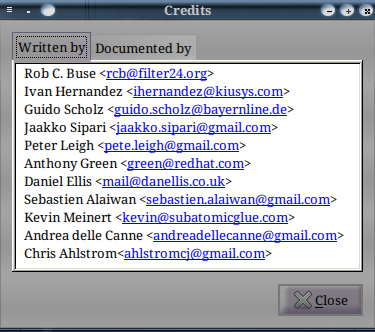
\includegraphics[scale=0.75]{menu/menu_help_credits.png}
   \caption{Help Credits}
   \label{fig:seq64_menu_help_credits}
\end{figure}

   Shows who has worked on the program, with the original author at the top
   of the list.

\begin{figure}[H]
   \centering 
   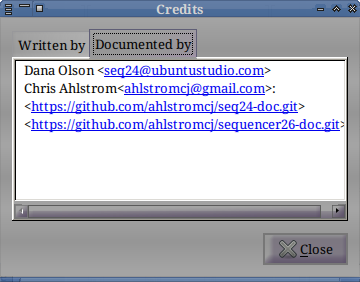
\includegraphics[scale=0.75]{menu/menu_help_doc.png}
   \caption{Help Documentation}
   \label{fig:seq64_menu_help_doc}
\end{figure}

   Shows who has documented this project.

\subsection{Menu / Help / Build Info...}
\label{subsec:seq64_menu_build_info}

   This menu entry shows the "Build Info" dialog.  This list of
   build options enabled in the current application is the same list
   that it generated via the one of the following command lines:

   \begin{verbatim}
      $ sequencer64 --version
      $ seq64 --version
   \end{verbatim}

\begin{figure}[H]
   \centering 
   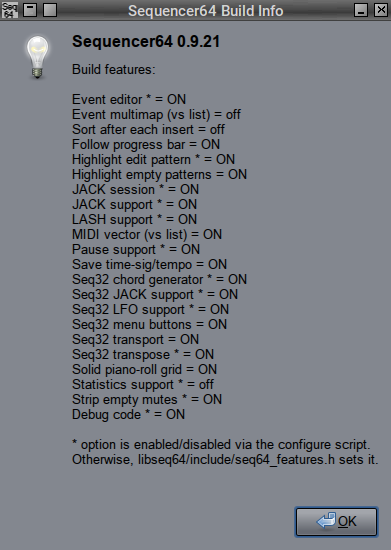
\includegraphics[scale=0.75]{new/menu_help_build_info.png}
   \caption{Help / Build Info}
   \label{fig:seq64_menu_help_build_info}
\end{figure}

%-------------------------------------------------------------------------------
% vim: ts=3 sw=3 et ft=tex
%-------------------------------------------------------------------------------
